\documentclass{article} % Tipo de documento

\usepackage{graphicx}
\usepackage{wrapfig}

\usepackage[utf8]{inputenc} % Permite el uso de caracteres del Español

\usepackage[T1]{fontenc}

% Carátula del Artículo  

\title{Reporte de Actividad 1}

\author{Diego Ivan Moreno Campa}

\date{30 de Enero, 2018}

% Comentario invisible

\begin{document}

\maketitle % Crea el título

\bigskip

\renewcommand{\abstractname}{Introducción}

\begin{abstract}

La atmósfera es una capa de gases, comúnmente conocido como aire, que cubre al planeta tierra y es retenida por su fuerza gravitacional. La atmósfera es importante para la vida en el planeta, ya que la protege de la radiación solar ultravioleta y tiene la presion necesaria para mantener agua liquida en la superficie terrestre.

En este artículo se desea explicar breve y claramente las propiedades y composición de la atmosfera terrestre.

\end{abstract}

\section{Composición}
El aire, y por lo tanto la atmósfera terrestre, es constituido mayormente por nitrógeno, oxígeno y argón. En general, la constitución de la atmósfera varía mucho localmente por las temperaturas y temporadas del lugar, como se muestra con el ejemplo de la concentración de agua, la cual varía dependiendo de la temperatura en las partes de la atmósfera.

\section{Estructura de la atmosfera}
\subsection{Capas principales}

La presión y la densidad de la atmósfera disminuye dependiendo de la altitud, sin embargo, la temperatura se mantiene relativamente constante. Gracias a que esta temperatura se puede medir, la atmósfera se puede categorizar en varias capas, lo que se conoce como estratificación de la atmósfera.
La atmosfera se divide en las siguientes capas:

\begin{itemize}
\item Exósfera: de 700 a 10,000 km 
\item Termósfera: de 80 a 700 km
\item Mesósfera: de 50 a 80 km
\item Stratósfera: de 12 a 50 km
\item Tropósfera: de 0 a 12 km
\end{itemize}

\subsection{Exósfera}

La exósfera es una capa que se extiende desde los 700 $km$ a 10,000 $km$, donde se mezcla con el viento solar. La exósfera esta compuesta por bajas densidades de hidrogeno, helio y nitrogen y dióxido de carbono en la parte baja, después de la exobase; estas bajas densidades permiten que una molecula no colisione con otra incluso si esta se lanza por varios kilometros y es por esto que los fenomenos climáticos no ocurren en la exosfera.

\subsection{Termósfera}
	
La termósfersa es una capa libre de vapor de agua que se extiende desde la mesopausa, a los 80 $km$, hasta la termopausa (también llamada exobase), a los 700 $km$ de altitud, aunque su altura varía considerablemente debido a los cambios de actividad solar. La parte baja de la termósfera que se extiende desde los 80 $km$ a los 550 $km$ es llamada ionósfera.

La temperatura de la termósfera aumenta gradualmente con la altura, la cual puede llegar a temperaturas de hasta 1500$^{\circ}$, sólo que esto no es muy significativo debido a que el aire a esa altura es bastante delgado, es por esto que una persona a esas alturas no sentiria el calor por las densidades tan bajas.

\subsection{Mesósfera}

\begin{wrapfigure}{r}{0.5\textwidth}
    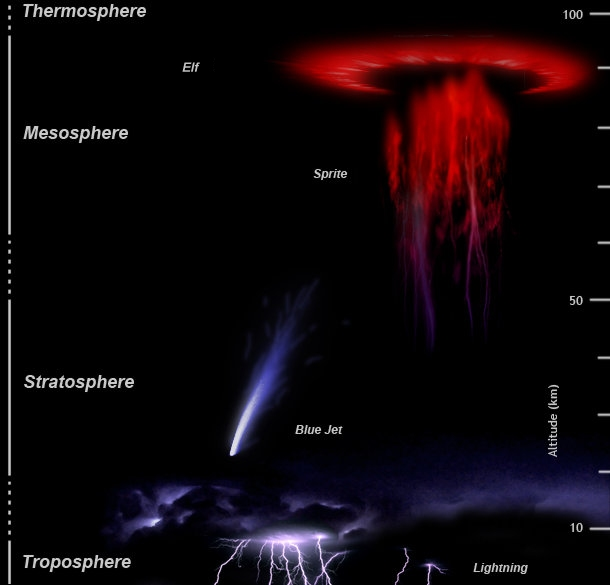
\includegraphics[height=5cm,width=0.50\textwidth]{Upperatmoslight1.jpg}
	\caption{Representación gráfica de un $hada$, un \textit{elfo} y un chorro azul (LTE's) encima de una cumulonimbus}
\end{wrapfigure}

La mesósfera se extiende desde la estratopausa a una altura de 50 $km$ a la mesopausa a 80 y 85 $km$.

Justo debajo de la mesopausa, como la temperatura es muy baja, el escaso vapor de agua se forma en nubes noctilucentes que son sólo visibles por el ojo humano entre una o dos horas antes del atardecer o despues del amanecer. Descargas inducidas por rayos conocidos como eventos luminosos transitoros (LTE's) se forman ocasionalmente en la mesósfera sobre cumulonimbus de la tropósfera. En esta capa también es en la que se desintegran los meteoros.

\newpage

\subsection{Estratósfera}

La estratósfera se extiende desde la tropopausa, a 12 $km$, hasta la estratopausa, a 50 y 55 $km$.

En la estratósfera se encuentra la capa de ozono donde ,como dice el nombre, es la parte en la que se encuentran concentraciones relativamente altas de esta molecula. En la estratósfera se encuentra una capa en la que la temperatura incrementa con la altitud debido a la absorción de radiación ultravioleta por la capa de ozono.

\subsection{Tropósfera}

La tropósfera se extiende desde la superficie terrestre a 12 $km$. La tropósfera esta limitada por la tropopausa en la cual se tiene una inversión de temperatura en la mayoria de las regiones, lo que significa que hay aire caliente encima de aire helado.

En general, la temperatura de la tropósfera disminuye conforme aumenta la altitud, debido a que se caliente la mayor parte por la superficie terrestre. La tropósfera además contiene alrededor del 80\% de la masa atmosférica, y debido a que se encuentra debajo varias capas exteriores, su densidad es la más grande entre las capas.

la característica principal de la tropósfera es el hecho de que es la capa con la mayoría cantidada de vapor de agua o humedad asi que es la capa en la que más ocurren fenómenos climáticos.

\subsection{Otras capas}
Entre las 5 capas principales que son clasificadas mayormente por su temperatura, las capas secundarias se clasifican por otras características: ~\\
~\indent La capa de ozono, como ya se menciono en la sección estratósfera, es una capa contenida mayormente en la estratósfera la cual se encuentran grandes concentraciones de ozono, por ende se le denomina la capa de ozono. Se extiende de 15 a 35 $km$ de altitud.~\\
\indent La ionósfera, como ya se menciono en la sección de Termósfera, se extiende desde los 50 $km$ a los 1,000 $km$ y es la capa en la que ocurren los fenómenos conocidos como aurora borealis o aurora australis. La ionósfera tiene aplicaciones prácticas porque afecta, por ejemplo, la propagación de radio ondas en la Tierra.~\\
\indent La homósfera y la heterósfera se determinan dependiendo de lo bien mezclados que se encuentren los gases atmosféricos. La homósfera se extiende desde la tropósfera hasta la parte de baja de la termósfera, donde la mezcla de los compuestos químicos no depende de la altura o el peso de los mismos compuestos. La heterosfera cubre la mayoría de la termósfera y toda la exósfera debido a que las concentraciones cambian con la altura.

\newpage

\section{Propiedades físicas}
\subsection{Presión y espesor}

\begin{wrapfigure}{l}{0.5\textwidth}
    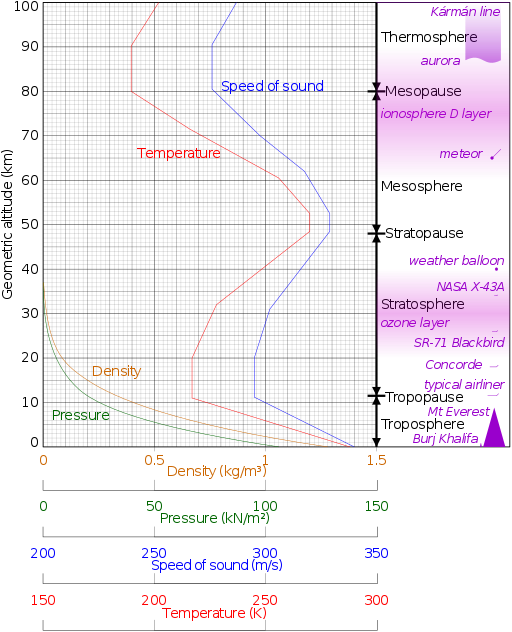
\includegraphics[height=5cm,width=0.50\textwidth]{AtmosModel.png}
	\caption{Comparación de la gráfica de la atmósfera estandar Estadounidense de altitud gráfica contra presión, densidad, temperatura y velocidad del sonido, junto a alturas aproximadas de varios objetos.}
\end{wrapfigure}
La presión atmosférica es el peso total del aire por unidad de área encima de donde se mide la presión.
La presión atmósferica al nivel del mar es 101,325 pascales definido por la atmósfera estandar internacional, un modelo atmosférico para describir como las propiedades físicas de la atmósfera cambian dependiendo de la altura. Sin embargo, la atmósfera se modela de una mejor manera con ecuaciones personalizadas para cada capa atmosférica.

\subsection{Temperatura y velocidad del sonido}

Como se ha mencionado anteriormente, el cambio o la distribución de temperatura varía en cada capa. Inicialmente disminuye la temperatura con la altitud después se estabiliza a los 11 $km$ y se mantiene asi hasta los 20 $km$ donde empieza a calentarse con la altitud debido a la capa de ozono.

Debido a que la velocidad del sonido depende únicamente de la temperatura, el cambio de la velocidad toma un perfil comparable al de la temperatura y no al de la densidad o la presión.

\subsection{Densidad y masa}

La densidad no se mide directamente, sino que se utiliza la ecuación del estado del aire. La densidad de la atmósfera disminuye conforme aumenta la altitud, lo cual se puede modelar usando la formula barometrica.

\newpage

\section{Propiedades ópticas}
\subsection{Dispersión}

Cuando la luz pasa a través de la atmósfera, los fotones interaccionan con la atmósfera por \textit{}dispersión.
Si la luz pasa directamente sin interaccionar se llama \textit{radiación directa}, mientras que cuando lo hace se llama \textit{radiación indirecta}. Un ejemplo de dispersión es la dispersión de Rayleigh, longitudes de onda mas cortas se dispersan más rapido que longitudes de onda mas largas, y es por esto que el cielo se ve azul. 
\subsection{Absorción}

Diferentes moléculas absorben distintas longitudes de onda de radiación. Cuando una molécula absorbe un fotón, la energía se incrementa y esto calienta a la atmósfera.

Esta absorción de parte de la atmósfera forma un espectro de absorción en la que solamente algunas longitudes de onda pueden escapar.
\subsection{Emisión}

La emisión es lo opuesto a absorción, ocurre cuando un objeto emite radiación, es la forma en la que la atmósfera se deshace de algo de calor absorbido. Los objetos tienden a emitir radiación dependiendo de sus curvas de emisión de cuerpo negro.

Debido a su temperatura, la atmósfera emite radiación infrarroja y es la razón por la que la superficie terrestre se enfría mejor en noches despejadas que en noches nubladas.

\subsection{índice de refracción}

El índice de refracción de la luz es cercano pero no exactamente 1, el indice de refracción depende de la temperatura, lo que da lugar a fenómenos de refracción cuando el gradiente de temperatura es alto.
Las variaciones sistemáticas del índice de refracción conllevan a la curvatura de rayos de luz a lo largo de caminos ópticos.

\newpage

\section{Circulación}

\begin{wrapfigure}{h}{0.5\textwidth}
    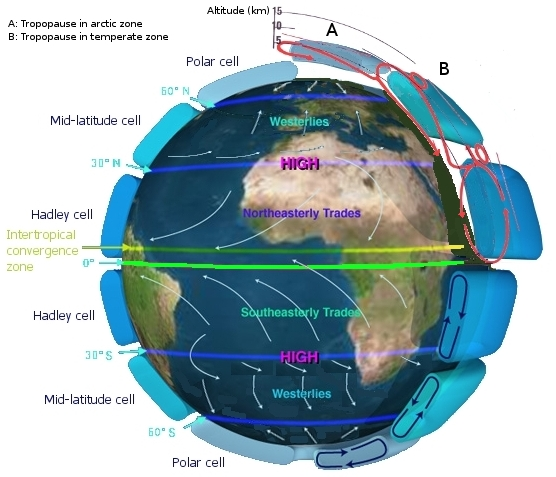
\includegraphics[height=5cm,width=0.50\textwidth]{Earth_Global_Circulation.jpg}
	\caption{Representación gráfica de la circulación de la Tierra a gran escala.}
\end{wrapfigure}

La circulación atmosférica es el movimiento a gran escala del aire a través de la tropósfera, y es la manera en la que se distribuye el calor alrededor del planeta. La circulación tiene una estructura relativamente constante debido a que depende de la rotación de la Tierra y la radiación del sol durante las temporadas.

A pesar de que la circulación se mantiene relativamente constante, los sistemas de clima a escalas más pequeñas ocurren aleatoriamente y predecciones distantes de estos no se pueden realizar en práctica antes de diez días, o en teoría menos de un mes.

\newpage

\section{Bibliografía}
Wikipedia (2018, January 29). Atmosphere of Earth.
\begin{verbatim}
https://en.wikipedia.org/wiki/Atmosphere_of_Earth
\end{verbatim}

\newpage

\title{Apéndice}

\begin{enumerate}
\item ¿Qué fue lo que más te llamó la atención de esta actividad? ~\\~\\
Lo que más me llamo la atención fue el uso de LaTeX para redactar una simple síntesis, esto me sirvió como introducción a LaTeX. El texto a sintetizar tuvo sus altas y bajas, recorde lo que era un LTE que son una de las cosas que me parecen más geniales.
\item ¿Qué fue lo que se te hizo menos interesante?~\\~\\
Debo decir que a pesar de que hubiera sido más eficiente crear un documento en Word pero entiendo el propósito de la práctica. no hay nada por qué quejarme, únicamente el hecho de que algunas partes de la síntesis me parecían dificil de sintetizar y creo que el hecho de que no tome información de otra fuente me dificulto este proceso.
\item ¿Qué cambios harías para mejorar esta actividad? ~\\~\\
Solo no restringir a sintetizar una página de WIkipedia, en lugar de eso pondría a sintetizar sobre un tema específico pero sin secciones especificas, si es que me doy a entender.
\item ¿Cuál es tu primera impresión de uso de LATEX?~\\~\\
Es muy rebuscado para realizar cosas simples como agregar imagenes, ordenar texto y agilizar la escritura, pero me puedo imaginar que LaTeX más bien sirve para crear plantillas y después editar en estas para tener una personalización o presentación agradable.
\item ¿El tiempo sugerido para esta actividad fue suficiente? ~\\~\\
Así es
\item ¿Encontraste algún documento o recurso en línea útil que quisieras compartir con los demás?  ~\\~\\
Desafortunadamente, yo no, solo utilice las referencias que se me proporcionaron
\end{enumerate}
       

\end{document}